\chapter{信号与槽}

信号(Signals)和槽(Slots)被用于在 Qt 对象之间通信。
信号槽机制是 Qt 的核心特性,同时也可能是与其他框架的类似特性区别最大的一部分。
信号槽使得 Qt 的元对象系统成为可能。

\section{介绍}

在 GUI 编程中,当我们修改某个控件后,我们通常希望另一个控件可以收到通知。
更普遍地,我们希望任何类型的对象都可以和另一个对象进行通信。
例如,如果用户点击了关闭按钮,我们可能希望该窗口的 close() 函数被调用。

其它开发工具中,使用回调来实现此类通信。
回调是指函数指针——当您希望某个处理函数通知您某些事件时,
通过传递一个函数指针(即回调)至该处理函数来实现,处理函数会在适合的时机调用这个回调。
尽管许多优秀的框架的确在使用此方法,但回调依然是一种非常不直观的手段,
而且可能会遭遇回调参数类型正确性校验等方面的问题。

\section{信号槽}

在 Qt 中,我们有回调技术的替代品:信号槽。信号会在特定事件发生时被发射;
Qt 的控件包含大量预定义的信号,并且我们也可以编写控件的子类来为它们添加自定义的信号。
槽是指会在响应对应信号时被自动调用的函数;Qt 的控件包含大量预定义的槽,并且,
编写控件的子类来添加自定义槽也是常见的做法,这样您便可以处理感兴趣的信号。

\begin{figure}[hbt!]  
\centering
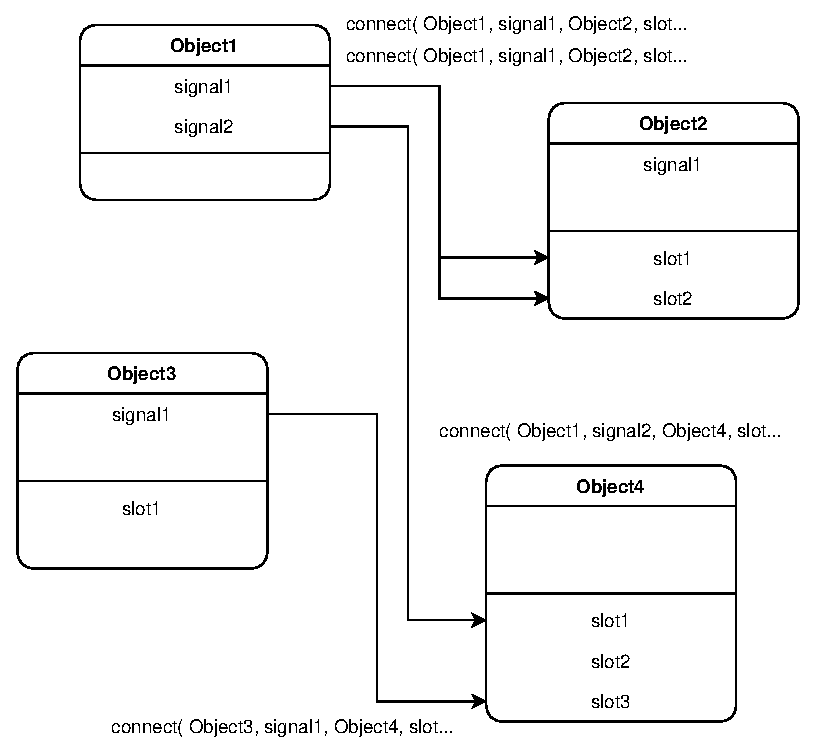
\includegraphics[width=0.5\textwidth]{eps/Signals_and_Slots.drawio.eps}
\end{figure}

信号槽机制是类型安全的:信号的函数签名必须与接收它的槽函数签名一致
(事实上,槽可以具有比它接收的信号更短的签名,因为允许忽略尾部的额外参数)。
鉴于函数签名需要兼容,当我们使用函数指针格式的 connect() 时,
编译器可以帮助我们识别它们的参数类型中的不匹配。
信号槽之间是松耦合关系:发射信号的类无需知晓也无需关心是哪个槽接收了这个信号。
Qt 的信号槽机制确保了,如果将一个信号连接至一个槽,
则槽会在正确的时机被调用,并传入信号所携带的参数。
信号槽可以携带任意类型、任意个数的参数,它们是完全类型安全的。

所有继承自 QObject 或它的任意子类型(如 QWidget)的类都可以包含信号槽。
对象在修改了可能会被其它对象感兴趣的状态时,会发射信号,
但并不需要知晓或关心是否有人接收了这个信号。这是真正的信息封装,
确保了该对象可以被当作软件中的一个组件所使用。

槽可被用于接收信号,但它们同时也是常规的成员函数。
正如一个对象并不知道是否有人接收了它的信号,
槽也不知道是否有信号连接至它。
这确保了 Qt 可以创建互相之间完全独立的组件。

将任意多的信号可以被连接至同一个槽,同一个信号也可以根据需要连接至任意多个槽。
甚至,将一个信号直接连接至另一个信号也是可行的(这会另第二个信号在第一个发射的同时被发射)。

两者结合后,信号槽构成了一种强大的组件化编程机制。

\section{信号}

当一个对象的内部状态被改变,同时它的使用者或所有者可能会感兴趣时,
它会发射信号。信号是类的公共成员函数,可以从任何地方发射,
但我们只推荐在定义这个信号的类和它的子类中发射。

当信号发射时,连接至它的槽通常会立刻执行,就如同常规的函数调用一样(即就地回调)。
此时,信号槽机制的运行完全独立于(即不依赖)任何 GUI 事件循环,
emit语句之后的代码会在所有槽函数返回后再继续执行。
此场景与队列连接有细微的差别——在后者中,
emit语句之后的代码会立即执行,而槽则会在随后才被调度。

若多个槽被连接至同一个信号,则当信号发射时,这些槽会按照连接的顺序依次执行。

信号会通过 moc 自动生成定义,不能在.cpp中手动编写定义。
信号不具备返回类型(即void)。(译者注:事实上,
非队列连接的信号可以具有返回类型,返回类型与槽返回类型相同,
也可用 QVariant 接收任意类型返回,但此机制不保证会被后续版本继续支持。
Qt 在 qobjectdefs\_impl.h 中,通过 operator, 
和 ApplyReturnValue 实现此机制,有兴趣的读者可自行查阅。)

关于函数参数:我们的经验是,若信号槽参数不使用特殊类型,
则可以具备更广的泛用性。如果 QScrollBar::valueChanged() 中使用了特殊类型,
假设命名为QScrollBar::Range,则它只能被连接至专门为 QScrollBar 设计的槽函数上,
而将不同的输入控件互相连接则是不可能的。


%%%%%%%%
\section{槽}

当连接至它的信号被发射时,槽会被调用。槽是常规的 C++ 函数,可以被正常调用;
它的特殊性质只有被连接至信号时才会体现。

由于槽是常规的成员函数(译者注:也可是静态成员函数或常规的全局函数),
当被直接调用时,它遵循标准的 C++ 规范。然而,作为槽,
它们可以被任何组件通过信号槽机制调用,而无视它的作用域。
这意味着从任意类的实例发射的信号,可以触发另一个非友元类实例中的私有槽。

您也可以将槽定义为虚函数,这在实践中被证明非常有用。

与回调相比,信号槽会稍微慢一些,因为它们提供了更多的灵活性,
不过在实际应用中这些性能差异通常无关紧要。一般来说,发射一个连接至槽的信号,
大约比直接调用接收者的函数慢上十倍(译者注:此处指函数调用的额外开销,
并非函数执行总耗时),此处不考虑虚函数调用开销。
这些开销被用于定位接收对象、线程安全地遍历所有连接(即检查接收者是否在发射过程中被销毁),
并将所有参数转换为规范化的形式。虽然十倍非虚函数的调用开销听起来很高,
但它其实比任何new或delete开销少得多。
例如,当执行一个字符串、向量或链表操作,而它们在内部依赖new或delete时,
信号槽开销在整个函数调用中只占据了一个非常小的比例。
这同样适用于在槽中执行系统调用,或在其中间接调用了超过十个函数的场景。
信号槽机制的简洁性和灵活性是值得付出这些开销的,并且您的用户甚至都无法感知到。

\begin{notice}
若其它库定义了名为signals或slots的类型(译者注:包括类型名称、函数签名、宏定义等任何代码标识),
将它们与 Qt 程序共同编译时会导致警告甚至错误。
为修复此问题,使用\#undef取消这些预编译符号的定义。
(译者注:不推荐此方法,建议使用下文的在 Qt 中使用第三方的信号槽机制)
\end{notice}

\section{一个小范例}

若有一个最小化的 C++ 类定义,如下所示:

\begin{cppcode}
 class Counter
 {
 public:
     Counter() { m_value = 0; }

     int value() const { return m_value; }
     void setValue(int value);

 private:
     int m_value;
 };
\end{cppcode}

则它对应的最小化的基于 QObject 的类型则为:

\begin{cppcode}
 #include <QObject>

class Counter : public QObject
{
	Q_OBJECT

public:
	Counter() { m_value = 0; }

	int value() const { return m_value; }

public slots:
	void setValue(int value);

signals:
	void valueChanged(int newValue);

private:
	int m_value;
};
\end{cppcode}

基于 QObject 的版本具备一些内部状态,并且提供了公共方法来获取这些状态,
同时还具备使用信号槽机制的组件化编程支持。
这个类可以通过发射 \hl{valueChanged()} 信号来通知外界它的状态发生了改变,
同时也拥有一个槽,让其它对象可以向其发送信号。

所有包含信号槽的类都必须在类的起始处声明 Q\_OBJECT ,并且必须继承自(直接或间接)QObject。
\hl{译者注:迄今所有版本中,QObject 均不支持虚继承和菱形继承,
即每个类只能拥有唯一一个非虚继承的 QObject 基类})

槽需要程序开发者提供定义,此处为Counter::setValue()槽的一个可能的定义:

\begin{cppcode}
void Counter::setValue(int value)
 {
     if (value != m_value) {
         m_value = value;
         emit valueChanged(value);
     }
 }
\end{cppcode}

emit 一行从该对象发射valueChanged()信号,并携带新的值作为参数。

在下方代码片段中,我们创建了两个Counter对象,使用 QObject::connect() 
将第一个对象的valueChanged()信号连接至第二个对象的setValue()槽。

\begin{cppcode}
Counter a, b;
QObject::connect(&a, &Counter::valueChanged,
                      &b, &Counter::setValue);

a.setValue(12);     // a.value() == 12, b.value() == 12
b.setValue(48);     // a.value() == 12, b.value() == 48
\end{cppcode}

调用a.setValue(12)会发射信号valueChanged(12),该信号被b的setValue()槽中接收,
即调用b.setValue(12)。然后b会发射相同的valueChanged()信号,
但由于没有槽被连接至b的valueChanged()信号,这个信号会被忽略。

注意,setValue()函数当且仅当value != m\_value时才会修改数值并发射信号。
这样避免了环形连接(如b.valueChanged()又被连接回a.setValue()时)时的无限循环。

默认下,每有一个连接,信号会被发射一次;若创建了两个连接,则信号会被发射两次。
您可以使用一次 disconnect() 来断开所有连接。
如果在连接时传递了 Qt::UniqueConnection 类型,
则连接只会被创建一次而非多次。如果已经有存在的重复连接(即对象的相同的信号,
被连接至相同对象的相同的槽),则新连接会失败并返回false。

本范例说明了,对象之间无需了解对彼此的任何信息,便可共同协作。
为实现此目的,对象们只需要通过一些简单的 connect() 调用连接至彼此,
或通过 uic 的自动连接特性完成。

\section{真实范例}

下文为一个简单的控件类的头文件范例,不包含成员函数。
此代码目为演示如何在您自己的应用中利用信号槽。

\begin{cppcode}
 #ifndef LCDNUMBER_H
 #define LCDNUMBER_H

 #include <QFrame>

 class LcdNumber : public QFrame
 {
     Q_OBJECT
\end{cppcode}

LcdNumber通过 QFrame 和 QWidget,间接继承自 QObject,后者提供了绝大部分信号槽特性。
这和内置的 QLCDNumber 控件有部分相似之处。

会被编译器展开为一些成员函数的声明,以供moc实现;
如果您遇到形如“无法解析的外部符号:LcdNumber”(undefined reference to vtable for LcdNumber)
的编译错误,那么您可能忘记执行moc,或忘记将moc输出包含到链接指令中。
(译者注:对于 qmake 工程,将包含 Q\_OBJECT 的头文件添加到 .pro 文件的 HEADERS 变量中,
即可自动执行 moc 并链接其输出)

\begin{cppcode}
 public:
     LcdNumber(QWidget *parent = nullptr);

 signals:
     void overflow();
\end{cppcode}

在类构造函数和公共成员之后,我们声明该类的信号。
当被要求显示不可能的数值时,LcdNumber类会发射信号overflow()。

如果不关心越界,或者知道不会发生越界,那么可以忽略overflow()信号,即不将它连接至任何槽。

另一方面,如果您想在数值溢出时调用两个不同的错误处理函数,只需简单地将信号连接至两个不同的槽。
Qt 会确保它们都被调用(按照连接的顺序)。

\begin{cppcode}
 public slots:
     void display(int num);
     void display(double num);
     void display(const QString &str);
     void setHexMode();
     void setDecMode();
     void setOctMode();
     void setBinMode();
     void setSmallDecimalPoint(bool point);
 };

 #endif
\end{cppcode}


槽是指接收信号的函数,用于获取其它控件状态改变的信息。
如上述代码所示,LcdNumber使用槽来设置被显示的数字。
由于display()同时也是该类在程序中的接口之一,这个槽是公共(public)的。

范例程序将 QScrollBar 的 valueChanged() 信号连接至此处的display()槽,
于是 LCD 数字会持续显示为滚动条的数值。

\begin{notice}
display()函数被重载;当连接信号至这个槽时,Qt 会选取适合的版本。在回调时,您需要自行查询多个不同的名称并跟踪它们的类型。
\end{notice}

\section{信号槽与默认参数}

信号槽可以包含默认参数,即具有默认值的参数。如 QObject::destroyed():

\begin{cppcode}
void destroyed(QObject* = nullptr);
\end{cppcode}

当一个 QObject 对象被删除时,它会发射 QObject::destroyed() 信号。
我们可以捕获此信号,此时我们可能仍持有被删除的 QObject 对象的悬空引用,
则可以将其清理掉。一个对应的槽函数签名可能为:

\begin{cppcode}
void objectDestroyed(QObject* obj = nullptr);
\end{cppcode}

为了将该信号连接至此槽,我们使用 QObject::connect()。有多种方式可以连接信号槽,首先是使用函数指针: